\chapter{Introducción}\label{cap1}
\section{Los problemas clásicos de levantamiento: extensión y clasificación}\label{sec:levext}
En distintos contextos matemáticos encontramos dos problemas básicos, común a todos ellos, si los despojamos de las características propias de un entorno: los problemas de extensión y levantamiento. \par

\subsection*{El problema de la extensión}\label{c1:ext}
Dado un diagrama de aplicaciones continuas 
$$
\begin{tikzcd}
	A \rar{f} \dar[hook]{i} & Y \\
	X \urar[dashed]{\tilde{f}}	&
\end{tikzcd} 
$$
donde $i$ es una ``inclusión'' en un contexto dado, ¿cuándo existe $\tilde{f}$, extensión de $f$? \par

La respuesta no es trivial. Es claro que, incluso si $i$ no es inclusión, ha de verificarse que si $i(a)= i(b)$ entonces $f(a) = f(b)$. Pero incluso si $i$ es biyectiva es necesario exigirle a $X$, para que la única $\tilde{f}$ posible sea continua, que posea la topología de la identificación determinada por $i$: 
$$
\theta \subset X \text{ es abierto si y sólo si } i^{-1} (\theta) \text{ es abierto de } A. 
$$
\newpage
Hay varios ejemplos de resultados que dan respuesta a este problema. Algunos dan una respuesta positiva:
\begin{teor} 
Si $X,Y$ son espacios métricos, $Y$ completo, y $A$ es denso en $X$, toda aplicación uniformemente continua $f:A\longrightarrow Y $ se extiende a una uniformemente continua $\tilde{f} : X \rightarrow Y$.
\end{teor} 

\begin{teor}[de Extensión de Tietze]
Sea $X$ normal, $A \subset X$ cerrado, $I \subset \mathbb{R}$ intervalo. Entonces toda $f : A \rightarrow I $  admite una extensión $\tilde{f} : X \rightarrow I$.
\end{teor}
\hypertarget{c1t:retractoh}{Mientras que la de otros es negativa:}
\begin{teor} \label{c1t:retracto}
La esfera $S^{n}$ no es un retracto del disco $D^{n+1}$. En otras palabras, la identidad $S^{n} \rightarrow S^{n}$ no se extiende a $D^{n+1}$.
\end{teor}

\subsection*{El problema del levantamiento}\label{c1:lev}
Dualmente \footnote{Dual en el sentido de ``Eckmann-Hilton'', dualidad que se definirá más adelante.},
nos encontramos con el problema del levantamiento de aplicaciones continuas. Es el siguiente: dado un diagrama
$$
\begin{tikzcd}
	{}	& X \dar[two heads]{p} \\
	Y \urar[dashed]{\tilde{f}} \rar{f} & B
\end{tikzcd}
$$
donde $p$ es sobreyectiva ¿cuándo existe $\tilde{f}$, levantamiento de $f$?\\ 
La respuesta tampoco es elemental. Incluso si $p$ es biyectiva hay que exigirle que sea homeomorfismo para que la única $\tilde{f}$ sea continua.\par

Igualmente hay resultados clásicos en distintos ambientes que contestan parcialmente esta cuestión.

\begin{teor} 
Sea $A \subset \mathbb{R}^2$ un conjunto estrellado respecto a $x_{0} \in A$ y $f : A \longrightarrow S^{1}$ una aplicación continua. Entonces f queda determinada de forma continua por su función angular, esto es, existe una aplicación $\tilde{f} : A \longrightarrow \mathbb{R}$ de tal forma que el siguiente diagrama es conmutativo:
$$
\begin{tikzcd}
	{}	& \mathbb{R} \dar{exp} \\
	A \urar{\tilde{f}} \rar{f} & S^1
\end{tikzcd}
$$
Esto es, $f(x) = (cos\tilde{f}(x), sen\tilde{f}(x))$. Es más, dos tales funciones $\tilde{f}$ se diferencian en un múltiplo entero de $2\pi$.
\end{teor}

Estos problemas son, en parte, origen de la teoria de homotopía. Muchas veces, los problemas de extensión y levantamiento son puramente homotópicos: \par
\begin{quotation}
Hay aplicaciones $p : X \longrightarrow B$ para las que existe el levantamiento de $f : \nobreak Y \longrightarrow B$ si existe el levantamiento de una ``deformada'' de $f$. \\
De igual forma existen algunas aplicaciones $i : A \longrightarrow X$ para las que existe una extensión de $g : A \longrightarrow Y$ si y sólo si existe alguna extensión para una ``deformada'' de g.
\end{quotation}
Introduzcamos el concepto de deformación en homotopía:
\begin{defin}
Dos aplicaciones $f, g : X \longrightarrow Y$ se dicen homótopas (deformables la una en la otra), denotado por $f \simeq g$, si existe  $H : X \times [0,1] \longrightarrow Y$ una aplicación tal que $H(x ,0) = f(x)$ y $H(x, 1) = g(x)$.
\end{defin}
Llegados a este punto, los problemas de extensión y levantamiento deparan ahora a un problema común de clasificación. ¿Cuándo dos aplicaciones $X \longrightarrow Y$ son homótopas? ¿Cómo es el conjunto $[X, Y]$ de clases de homotopía de aplicaciones $X \longrightarrow Y$? \par 
Los métodos que se siguen son, a grosso modo, de dos enfoques distintos:\\
Por una parte, a los espacios se le asocian modelos algebraicos y morfismos entre los respectivos modelos algebraicos a las aplicaciones. Estas asociaciones permiten parcialmente su clasificación. \par 
Como ejemplo, probemos el \hyperlink{c1t:retractoh}{teorema anterior} por el que $S^n$ no es un retracto de $D^{n+1}$. Para ello, asociemos a $S^n$ un invariante algebraico no nulo (como por ejemplo el grupo de homología $n$-ésimo). Como el disco $D^{n+1}$ es deformable a un punto, todos esos invariantes se hacen 0. Si $S^n$ fuese retracto de $D^{n+1}$ existiría un diagrama como el siguiente:
$$
\begin{tikzcd}
	S^n \arrow{rr}{Id_{S^n}} \drar{i} & & S^n \\
		&	D^{n+1} \urar{r} & 
\end{tikzcd}
$$
que algebraicamente daría lugar a 
$$
\begin{tikzcd}
	0 \neq F(S^n) \arrow{rr}{Id} \drar & &  F(S^n) \neq 0 \\
		&	0 \urar & 
\end{tikzcd}
$$
lo que resulta contradictorio. \par

Por otra parte, para saber más sobre $[X, Y]$ es habitual tratar de dotar a este conjunto de otras estructuras (grupo, módulo...) que den luz sobre su comportamiento. 

\section{Homotopía: Nociones básicas}\label{sec:homotbas}
La relación de homotopía es básica y formaliza la noción de deformación continua de dos espacios: dos aplicaciones $f, g : X\longrightarrow Y$ son homótopas si existe $H : X \times I \longrightarrow Y$ tal que $H(x, 0) = f(x)$, $H(x, 1) = g(x)$. 
\begin{prop}
La relación de homotopía es una relación de equivalencia en el conjunto de aplicaciones continuas de $X$ a $Y$.
\end{prop}
\begin{demo} 
La propiedad reflexiva es clara sin más que tomar la aplicación $F(x,t) = x$.\\
Para la simétrica, si $H : f \simeq g$ entonces $F : X \times I \longrightarrow Y$, $F(x, t) = H(x, 1-t)$ es una homotopía de $g$ a $f$.\\
Veamos ahora la transitiva. Si $F : f \simeq g$, $H : g \simeq h$ entonces $G : X \times I \longrightarrow Y$,

$$G(x, t) = 
\begin{cases}
	F(x, 2t) 	& 	\text{ si } t \leq \frac{1}{2}\\
	H(x, 2t - 1)& 	\text{ si } t \geq \frac{1}{2}
\end{cases}$$ 
es una homotopía de $f$ a $h$.
\end{demo}
\begin{ejems}
\begin{enumerate}
\item \label{ej1:1} Cuando $X = I$, esto es, al trabajar con curvas, se observa mejor la deformación:
\begin{figure}[h]
\centering
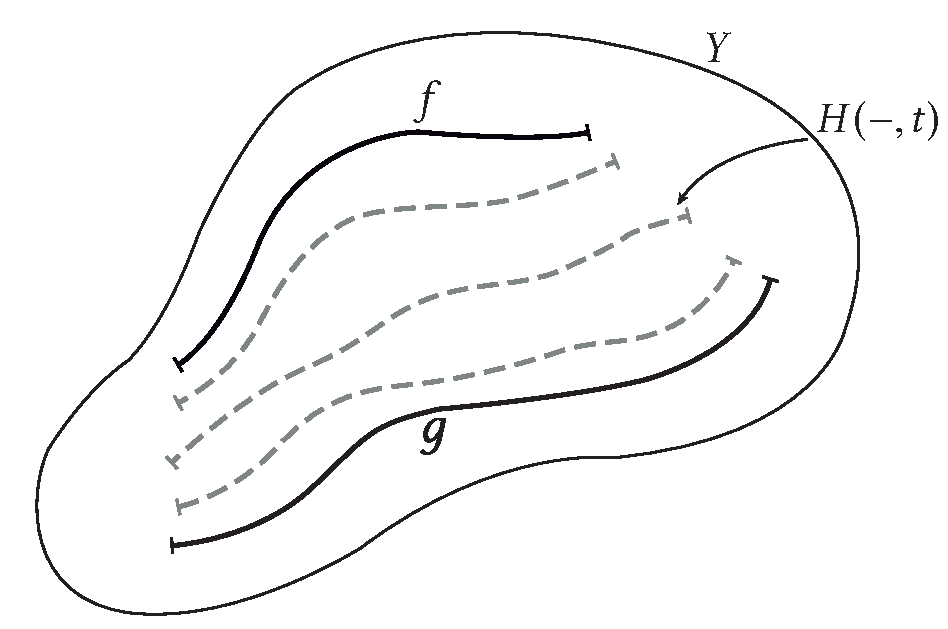
\includegraphics[width=0.4\textwidth]{images/homotcamin.pdf}
\end{figure}
\item \label{ej1:2} Sean $X = Y = \mathbb{R}^n$, y consideremos las aplicaciones $f = Id_{\mathbb{R}^n}$ y $g \equiv 0$. Entonces $f \simeq g$ mediante la aplicación
$$H : \mathbb{R}^n \times I \longrightarrow \mathbb{R}^n$$ $$H(x, t) = tx$$
\end{enumerate}
\end{ejems}
A menudo estamos interesados en aplicaciones entre pares
$$f : (X, A) \longrightarrow (Y, B)$$ que no es más que una aplicación continua tal que $f(A) \subset B$. En este caso, $f, g : (X, A) \longrightarrow (Y, B)$ son homótopas si existe $H : X \times I \longrightarrow Y$ tal que $\forall t \in I$, $H_t = \nobreak H(-, t) : (X, A) \longrightarrow (Y, B)$.\par
Un caso particular de suma importancia es el de los espacios punteados $(X, x_0)$. En este caso, $f \simeq g : (X, x_0) \longrightarrow (Y, y_0)$ si existe $H: X \times I \longrightarrow Y$ tal que $H(x, 0) = f(x), H(x, 1) = g(x)$ y $H(x_0, t) = y_0$ $\forall t \in I$.\\
\begin{ejems}
\begin{enumerate}
\item \label{ej2:1} En el ejemplo anterior \ref{ej1:2}, podemos considerar $f \simeq g : (\mathbb{R}^n, 0) \longrightarrow (\mathbb{R}^n, 0)$ tomando como homotopía la misma función $H$.

\item \label{ej2:2} Si consideramos un espacio como el siguiente: \\
\begin{tabular}{ll}
\begin{minipage}{0.5\textwidth}
Tenemos que $f : I \longrightarrow Y$ es obviamente homótopa a la constante en $y_0$ que denominamos $c_{y_0}$. Pero la aplicación de pares $f : (I, \{ 0,1 \}) \longrightarrow (Y, y_0)$ no es homótopa a la constante $c_{y_0}$.
\end{minipage}
&
\begin{minipage}{0.5\textwidth}
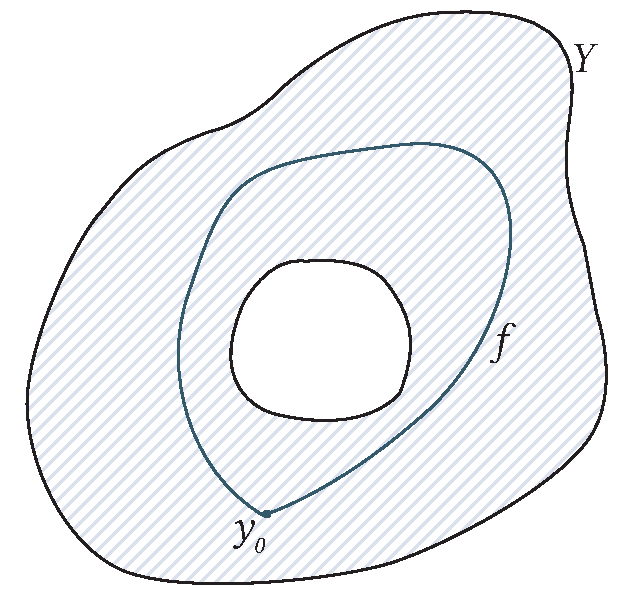
\includegraphics[width=0.65\textwidth]{images/homotrelatalt.pdf}
\end{minipage}
\end{tabular}

\item \label{ej2:3} Dado $E^2 = \{ x \in \mathbb{R}^2 : \| x \| \leq 1 \}$, tenemos que $Id \simeq a$ donde $a$ es la función antípoda mediante la hopotopía de la rotación: $H : E^2 \times I \longrightarrow E^2$ dada por $H(x, t) = H(\rho e^{i\theta}, t) = \rho e^{i(\theta + t\pi)}$ \par
\begin{figure}[h]
\centering
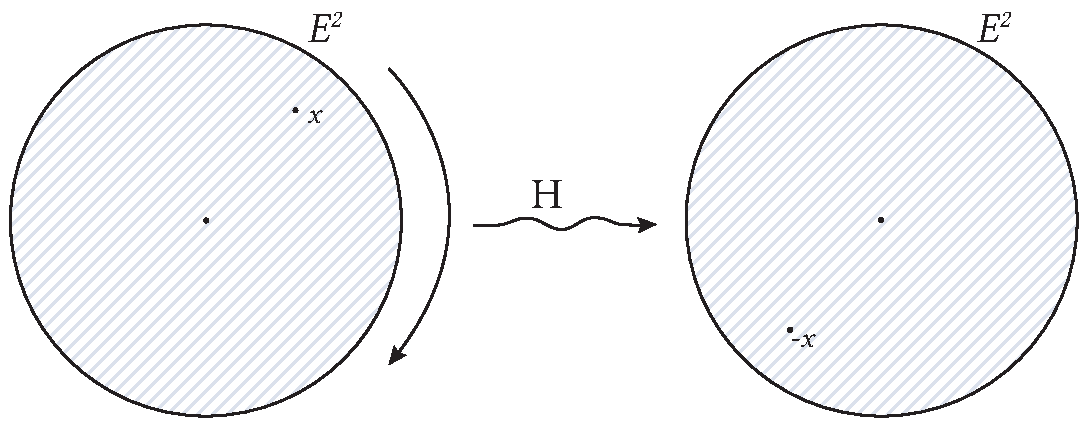
\includegraphics[width=0.65\linewidth]{images/homotrotacalt.pdf}
\end{figure}
Es más, como aplicaciones de pares, $Id \simeq a$ mediante $H : (E^2, S^1) \times I \longrightarrow (E^2, S^1)$. Sin embargo, $\nexists \, x_0 \neq 0$ tal que $Id \simeq a$ como aplicaciones $(E^2, x_0) \longrightarrow (E^2, -x_0)$.
\end{enumerate}
\end{ejems}
Al conjunto cociente formado por las clases de homotopía de aplicaciones continuas de $(X, A)$ en $(Y, B)$ se le denota por $[(X, A), (Y, B)]$.\\
Por tanto, ya podemos definir nuestros ``objetos deformables''.
\begin{defin}
Dos espacios $X$ e $Y$ son homotópicamente equivalentes si existen aplicaciones $f: X \longrightarrow Y$ y $g: Y \longrightarrow X$ tales que $g \circ f \simeq 1_X$ y $f \circ g \simeq 1_Y$. A las aplicaciones $f$ y $g$ se les denomina equivalencias de homotopía.
\end{defin}

\begin{ejems}
\begin{enumerate}
\item \label{ej3:ret} \textbf{Retractos}: 
\begin{tikzcd}
A \rar[hook]{i} & X  
\end{tikzcd}
es un retracto de X si existe una aplicación $r : X \longrightarrow A$ tal que $r \circ i = 1_A$.
Decimos que $A$ es un retracto de deformación de $X$ si además $i \circ r \simeq 1_X$.\\
Como ejemplo, $S^n = \{ x \in \mathbb{R}^{n+1}$ : $\| x \| = 1 \}$ es un retracto de deformación de $\mathbb{R}^{n+1} -\{ 0 \}$. En efecto, si consideramos 
\begin{align*}
r : \mathbb{R}^{n+1} &-\{ 0 \} \longrightarrow S^n \\
x &\longmapsto \frac{x}{\| x \|}
\end{align*}
entonces 
\begin{align*}
H : \mathbb{R}^{n+1} &-\{ 0 \} \times I \longrightarrow \mathbb{R}^{n+1} -\{ 0 \} \\
H(x, t) &= (1 - t)x + \frac{tx}{\| x \|} 
\end{align*}
es una homotopía entre $Id_{\mathbb{R}^{n+1} -\{ 0 \}}$ e $i \circ r$.

\item \label{ej3:contr} \textbf{Espacios contráctiles}: Un espacio X es contráctil si tiene el mismo tipo de homotopía de un punto, o equivalentemente, la identidad en $X$ es homótopa a una constante, o un punto es retracto de deformación del espacio. Antes hemos visto que $\mathbb{R}^n \simeq \ast \simeq D^n $.

\item \label{ej3:peine} \textbf{El espacio peine} P es un espacio contráctil. P es el conjunto definido de la siguiente forma: 

\begin{tabular}{ll}
\begin{minipage}{0.3\textwidth}
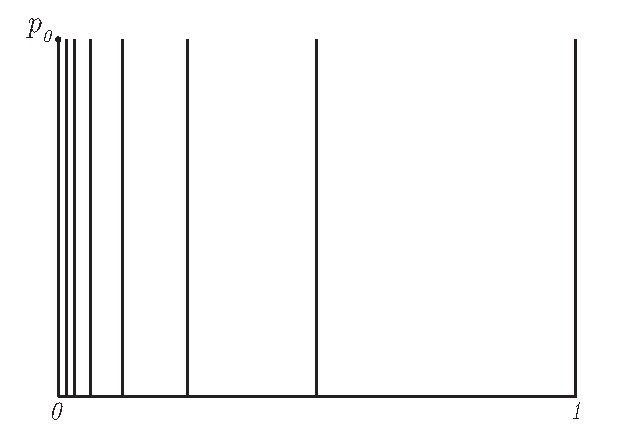
\includegraphics[width=\textwidth]{images/peine.pdf}
\end{minipage}
&
\begin{minipage}{0.6\textwidth}
\[ P = \bigcup_{n=1}^\infty \left( \left\lbrace \frac{1}{n} \right\rbrace \times [0, 1]\right) \cup \{ 0 \} \times [0, 1] \cup [0, 1] \times \{ 0 \} \]
que obviamente es contráctil, aunque $Id_P \not \simeq_{p_0} c_{p_0}$ para un $p_0 \notin [0, 1] \times \nobreak \{ 0 \} $.
\end{minipage}
\end{tabular}
\end{enumerate}

\end{ejems}
Relacionado con el ejemplo \ref{ej3:contr} y con el problema de la extensión tenemos el siguiente resultado:\\
\begin{teor}
Sea $f : S^n \longrightarrow X$ una aplicación continua. Entonces $f \simeq \ast$ si y sólo si $f$ se extiende al disco. 
\[
\begin{tikzcd}
	S^n \arrow{rr}{f} \drar[hook] & & X \\
		& D^{n+1} \urar{\tilde{f}}
\end{tikzcd}
\]
\end{teor}
\begin{demo}
Supongamos $H : f \simeq c_{x_0}$. Definimos entonces $\tilde{f} : E^{n+1} \longrightarrow X$ dada por:
\[
\tilde{f}(p )= 
\begin{cases}
	x_0 & \text{ si }\| p \| \leq \frac{1}{2} \\
	H(\frac{p}{\| p \|}, 2 - 2\| p \|) & \text{ si } \| p \| \geq \frac{1}{2}
\end{cases}
\]
que es la extensión que queríamos.

Recíprocamente, si $\tilde{f}$ es una extensión, $H(x, t) = \tilde{f}((1 - t)x)$ es una homotopía de $f$ a la constante. 
\end{demo}

\subsection{Espacios comúnmente utilizados}\label{c1:espcomun}
Algunas de las construcciones que serán de utilidad son las siguientes:
\begin{itemize}
\item \hypertarget{ecom:prod}{\textbf{El producto de espacios}} $X \times Y$ \\

\item \hypertarget{ecom:suma}{\textbf{La suma puntual}} o ``wedge'', denotado por $X \vee Y$ que puede verse como el conjunto cociente $X \dot\cup Y \Bign/ x_0 \sim \nobreak y_0$ o como un subconjunto de  $X \times Y$, esto es, $X \vee Y = X \times \{y_0\} \cup \{x_0\} \times Y$\\

\item \hypertarget{ecom:smash}{\textbf{El smash}} definido como $X \wedge Y = X \times Y \Bign/ X \vee Y$. Esto es, el producto en el que identificamos ``los ejes'' a un punto.\\


\begin{tabular}{ll}
\begin{minipage}{0.5\textwidth}
\item \hypertarget{ecom:cono}{\textbf{El cono de $X$.}} Dado $X$, el cono de $X$ se define como $CX = \faktor{X \times I}{X \times \{0\}}$.\\
Si queremos ``puntearlo'', hacemos además
\[CX = \faktor{X \times I}{X \times \{ 0 \} \cup \{ x_0 \} \times I} \] 
\end{minipage}
&
\begin{minipage}{0.5\textwidth}
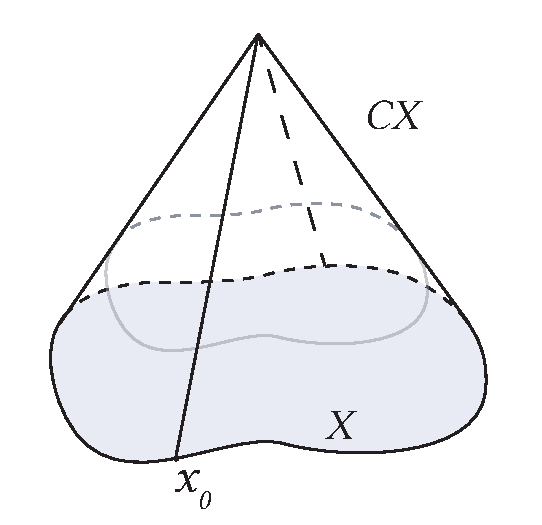
\includegraphics[width=0.6\textwidth]{images/conox.pdf}
\end{minipage}
\end{tabular}
 
 y el punto base es $[x_0, t]$. Claramente la aplicación 
\begin{align*}
X &\longhookrightarrow CX \\ 
x &\longmapsto [(x, 1)]
\end{align*}
es un homeomorfismo en su imagen por lo que podemos pensar en $X$ como un subespacio del cono. Además $CX$ es contráctil.
\end{itemize}
\subsection{Adjuntando celdas o cómo pegar un disco a un espacio}\label{c1:unionceldas}
Sea $X$ un espacio topológico y $E^n$ un disco de dimensión $n \geq 1$. \\
 Sea $f : S^{n-1} \longrightarrow X$ una aplicación continua. Definimos $X \cup_f e^n$, el espacio obtenido adjuntando a X una $n$-celda mediante $f$: \par
\begin{tabular}{ll}
\begin{minipage}{0.5\textwidth}
\[ X \cup_f e^n := \faktor{ X \dot{\cup} E^n}{ \sim} \]
\end{minipage}
&
\begin{minipage}{0.5\textwidth}
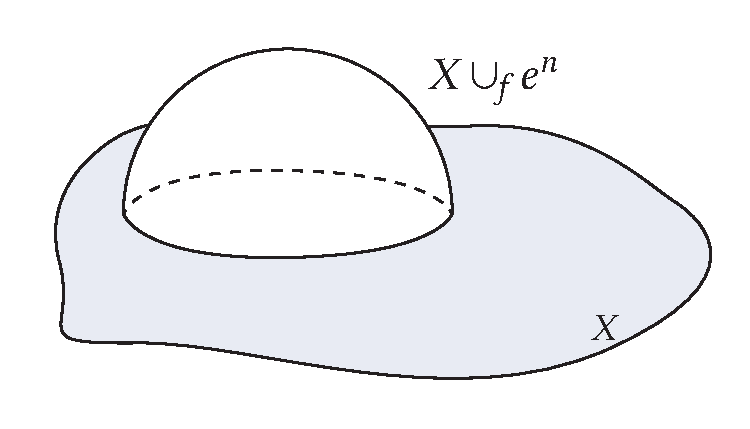
\includegraphics[width=0.8\textwidth]{images/uceldas.pdf}
\end{minipage}
\end{tabular}


donde $\sim$ es la menor relación de equivalencia que contiene a $x \in S^{n-1} \sim f(x)$\\

\begin{prop}
La adjunción de una celda sólo depende del tipo de homotopía de la aplicación de adjunción.
\end{prop}
\begin{demo}
Sean $f ,g : S^{n-1} \longrightarrow X$ dos funciones con el mismo tipo de homotopía, $f \simeq g$. Veamos que entonces que $X \cup_f e^n \simeq X \cup_g e^n$.\par 
Si $H : f \simeq g$, definimos las siguientes funciones:
$$k : X \cup_f e^n \longrightarrow X \cup_g e^n
\text{ dada por }
k(x) = 
\begin{cases}
	x  & \text{si } x \in X \\
	2x & \text{si } x \in e^n$, $\| x \| \leq \frac{1}{2} \\
	H(\frac{x}{\| x \|}, 2 - 2\|x\|) & \text{si } \| x \| \geq \frac{1}{2}
\end{cases}$$ 
$$h : X\cup_g e^n \longrightarrow X \cup_f e^n
\text{ dada por }
h(x) = 
\begin{cases}
	x  & \text{si } x \in X \\
	2x & \text{si } x \in e^n$, $ \| x \| \leq \frac{1}{2} \\
	H(\frac{x}{\| x \|}, 2\| x \| - 1 & \text{si } \| x \| \geq \frac{1}{2}\\
\end{cases}$$
Y tenemos que $h \circ k \simeq 1_{X \cup_f e^n}$ mediante la función $F : X \cup_f e^n \times I \longrightarrow X \cup_f e^n$ dada por: \\
\begin{center}
$F(x,t) = 
\begin{cases}
	x  & \text{si } x \in X \\
	4x & \text{si } \| x \| \leq \frac{1}{4} \\
	H(\frac{x}{\| x \|}, (4\|x\| - 1)t) & \text{si } \frac{1}{4} \leq \| x \| \leq \frac{1}{2} \\
	H(\frac{x}{\| x \|}, (2 - 2\|x\|)t) & \text{si } \| x \| \geq \frac{1}{2}
\end{cases}$ \\
\end{center}
De forma análoga se prueba que $k \circ h \simeq 1_{X \cup_g e^n}$.
\end{demo}
\textbf{Consecuencia:} Si $X$ es arcoconexo, $X \cup_f e^1 \simeq X \vee S^1$ y si $f \simeq \ast$, entonces
$X \cup_f e^n \simeq X \vee S^n$. \\


\begin{teor}
Una aplicación $f : (X, x_0) \longrightarrow (Y, y_0)$ es null-homótopa si y sólo si se extiende a $CX$: 
$$
\begin{tikzcd}
	X \arrow{rr}{f} \drar[hook] & & Y \\
	& CX \urar[dashed]{h} & 
\end{tikzcd}
$$
\end{teor}
\begin{demo}
Sea $H : f \simeq c_{y_0}$ una homotopía. Definimos entonces la aplicación $h : CX \longrightarrow Y$, dada por $h([x, t]) = H(x, t)$. Está bien definida, ya que $H(X \times \{ 0 \} \cup \{ x_0 \} \times I) = y_0$ y se extiende a $f$.\par 
Recíprocamente, dada $h : (CX, \ast) \longrightarrow (Y, y_0)$ extensión de $f$, definimos $H: X \times I \longrightarrow Y$ como $H = h \circ \pi$ (donde $\pi: X \times I \longrightarrow CX$ es la proyección canónica) y se tiene que 
$H(x, 0) = y_0$, $H(x, 1) = f(x)$ y $H(x_0, t) = y_0$.
\end{demo}

\section{Suspensión y lazos de un espacio}\label{sec:suspylazos}

Como ya hemos visto, el \hyperlink{ecom:cono}{cono de $X$}, $CX$, es el espacio contráctil $CX = \faktor{X \times I }{X \times \{ 0 \}}$. De igual forma, la suspensión de $X$, denotada por $\Sigma X$, se define como \par 
\begin{tabular}{ll}
\begin{minipage}{0.5\textwidth}
\[ \Sigma X =  \faktor{X \times I}
{ \footnotesize{\begin{matrix}
(x, 1) \sim (x', 1) \\
(x, 0) \sim (x', 0)
\end{matrix}}} \] 
\end{minipage}
&
\begin{minipage}{0.5\textwidth}
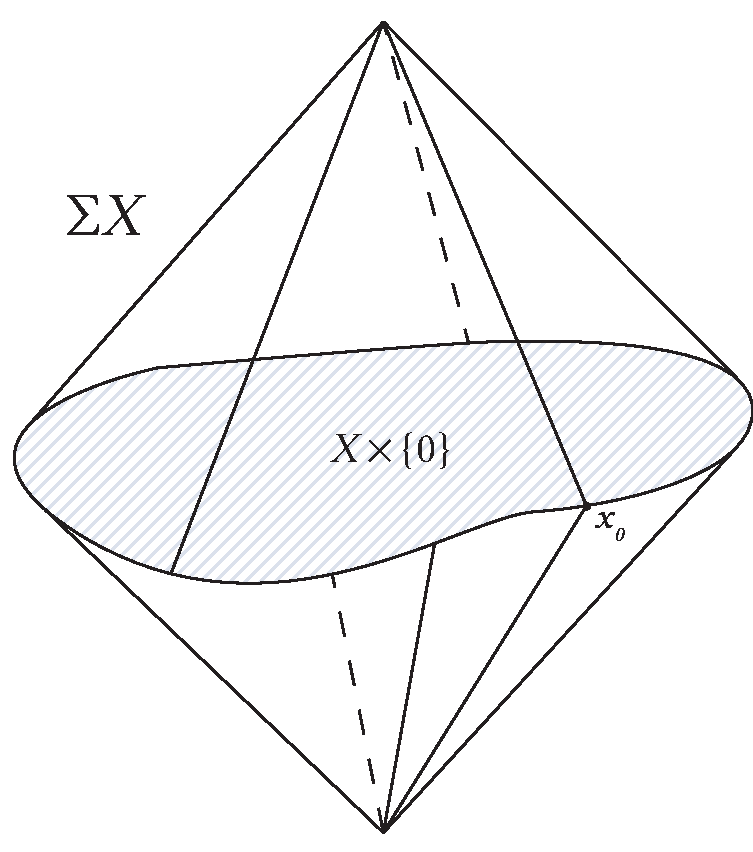
\includegraphics[width=0.6\textwidth]{images/suspensionalt.pdf}
\end{minipage}
\end{tabular}
Si $x_0$ es el punto base de $X$, el cono punteado era
\[ CX = \faktor{X \times I}{X \times \{ 1 \}  \cup \{ x_0 \} \times I}\]
De igual forma la suspensión punteada es 
\[ \Sigma X = \faktor{ X \times I }
{\footnotesize{ \begin{matrix}
(x, 1) \sim (x', 1) \\ 
(x, 0) \sim (x', 0) \\ 
(x_0, t) \sim (x_0, t')
\end{matrix} }} \]
Obviamente, si a $I$ le damos la estructura de $CW$-complejo con dos $0$-celdas $\{0\}, \{1\}$ y una $1$-celda, tanto el cono $CX$ como la suspensión $\Sigma X$ (que no es más que $CX \Bign/ X \times \{ 0 \}$) tienen estructura de $CW$-complejo. Nótese además que toda aplicación $f : X \rightarrow Y$ se puede suspender $\Sigma f : \Sigma X \rightarrow \Sigma Y$ de forma obvia:
$\Sigma f [x, t] = [f(x), t]$. \par

Por otro lado tenemos los lazos en un espacio topológico punteado $(X, x_0)$ que se definen como
\begin{align*}
\Omega X =& (X, x_0)^{(S^1, p_0)} = \{ f : S^1 \rightarrow X : f(p_0)  = x_0 \} \\ 
=& \{ f : I \rightarrow X : f(0) = f(1) = x_0 \}
\end{align*}
$\Omega X$ resulta ser $CW$-complejo si $X$ lo es. $\Omega X$ está punteado por la constante en $x_0$, $c_{x_0}$. Se tiene entonces: 
\begin{teor}
Para cualesquiera espacios punteados $X$ e  $Y$ se tiene que 
\begin{center}
$[\Sigma X, Y ] \cong [X, \Omega Y]$ \footnote{Siempre que escribamos clases de homotopía, nos referiremos a espacios punteados.}
\end{center}
\end{teor}
\begin{demo}
En general, el conjunto de aplicaciones continuas 

\[ (Y, y_0)^{(\Sigma X, \ast)} \cong (\Omega Y, \ast)^{(X, x_0)} \]

En efecto, la aplicación

\[ \varphi : (\Omega Y, \ast)^{(X, x_0)} \rightarrow (Y, y_0)^{(\Sigma X, \ast)} \]
dada por 
\begin{align*}
\varphi (g) : \Sigma X \longrightarrow Y \\
\varphi (g)[x, t] = g(x)(t)
\end{align*} 
está bien definida y tiene por inversa a 
\[ \varphi^{-1} : (Y, y_0)^{(\Sigma X, \ast)} \rightarrow (\Omega Y, \ast)^{(X, x_0)} \]
\begin{align*}
\varphi^{-1} (f)& : X \rightarrow \Omega Y \\
\varphi^{-1}(f)&(x)(t) = f[x, t]
\end{align*}
Veamos que $\varphi$ induce una aplicación $\bar{\varphi} : [X, \Omega Y] \rightarrow [\Sigma X, Y] $ para lo que hemos de ver que si $f \simeq_{\{ x_0 \}} g$ entonces $\varphi (f) \simeq_{\ast} \varphi (g)$. \par
Sabemos pues que existe una homotopía $H: X \times I \rightarrow \Omega Y$ tal que $H(x,0) = f(x) $, $H(x,1) = g(x)$ y 
$H(x_0, t) = c_{y_0}$ $\forall t \in I$.\\
Definimos entonces 
\begin{align*}
F: \Sigma X \times I &\longrightarrow Y \\
F([x,t],s) &= H(x,s)(t) \\
F([x,t],0) &= H(x,0)(t) = f(x)(t) = \varphi(f)[x,t] \\
F([x,t], 1) &= \varphi(g)[x,t]_j \\
F([x_0,t],s) &= H(x_0, s)(t) = y_0
\end{align*}
que es una homotopía entre $\varphi (f)$ y $\varphi (g)$.
De igual forma $\varphi^{-1}$ induce $\overline{\varphi^{-1}} : [\Sigma X, Y] \rightarrow [X, \Omega Y]$ y $\bar{\varphi}^{-1} = \overline{\varphi^{-1}}$\\
\end{demo}

\textbf{Nota:} $\Omega$ y $\Sigma$ son duales en el sentido de Eckman-Hilton.\\

\noindent En $\Sigma X$ podemos definir la operación  $\mu : \Omega X \times \Omega X \longrightarrow \nobreak \Omega X$
\[
\mu(\omega, \omega')(t) = 
\left\{ \begin{array}{ll}
             \omega(2t)		&   $si $ t \leq \frac{1}{2} \\
             \omega'(2t-1)	&   $si $ t \geq \frac{1}{2} \\
        \end{array}
\right.
\]
$\mu(\omega, \omega')$ está bien definida y para ver que es continua basta ver
\begin{align*}
\Omega X \times \Omega X \times I &\longrightarrow \Omega X \times I \longrightarrow X \\
(\omega, \omega', t) &\longmapsto 
\left\{ \begin{array}{ll}
             \omega(2t)		&  t \leq \frac{1}{2} \\
             \omega'(2t-1)	&  t \geq \frac{1}{2} \\
        \end{array}
\right.
\end{align*}
que obviamente es continua. \\
Esta operación permite definir otra en $[X, \Omega Y]$, dada por 
\[ (f \cdotp g)(x) = f(x) \cdotp g(x) = \mu(f(x), g(x)) \]

Veamos que $\mu$ hace de $\Omega Y$ un ``grupo homotópico'', esto es, un H-grupo. Demostremos la siguiente proposición:
\begin{prop}
Consideremos el espacio de los lazos $\Omega Y$. Entonces
\begin{enumerate}
\item $c_{y_0}$ es el neutro homotópico.
\item $\mu$ es homotópicamente asociativa.
\item Si $\omega \in \Omega Y$, entonces el inverso homotópico de $\omega$ es $\omega^{-1}(t) = \omega(1 - t)$.
\end{enumerate}
\end{prop}
\begin{demo}
\begin{enumerate}
\item Veamos que $c_{y_0}$ es neutro por la derecha. Consideramos
\begin{align*}
\mu(-,c_{y_0}) : \Omega Y &\longrightarrow \Omega Y \\
\omega &\longmapsto \omega \cdotp c_{y_0}
\end{align*}
y tenemos que ver que es homótopa a la identidad. Para ello basta considerar la homotopía
\begin{align*}
F: \Omega Y \times I \longrightarrow \Omega Y \\
F(\omega, t)(s) = 
\begin{cases}
\omega\left(\frac{2s}{t+1}\right) & 0 \leq s \leq \frac{t+1}{2} \\
y_0													& \frac{t+1}{2} \leq s \leq 1
\end{cases}
\end{align*}
Igualmente se demuestra que $\mu(c_{y_0}, -) \simeq Id_{\Omega Y}$.
\item Para ver que $\mu$ es asociativa, tenemos que ver que el siguiente diagrama es homotópicamente conmutativo: 
\[
\begin{tikzcd}
	\Omega Y \times \Omega Y \times \Omega Y \rar{\mu \times Id_{\Omega Y}} \dar{Id_{\Omega Y} \times \mu}
		  & \Omega Y \times \Omega Y \dar{\mu} \\
	\Omega Y \times \Omega Y \rar{\mu} 
		  & \Omega Y
\end{tikzcd}
\]
La homotopía necesaria para esto es:
\begin{align*}
G: 	\Omega Y &\times \Omega Y \times \Omega Y \times I \longrightarrow \Omega Y \\
G(\omega, \omega' \omega'', t)(s) &= 
\begin{cases}
\omega \left( \frac{4s}{t+1}\right) & 0 \leq s \leq \frac{t+1}{4} \\
\omega'(4s - t - 1)         		 & \frac{t+1}{4} \leq s \leq \frac{t+2}{2} \\
\omega''\left( \frac{4s -2 - t}{2-t}\right) & \frac{t+2}{4} \leq s \leq 1
\end{cases}
\end{align*}

\item Por último definimos el morfismo inverso $\varPhi : \Omega Y \longrightarrow \Omega Y $ dado por $\varPhi(\omega) = \omega^{-1}$. Tenemos que ver que $\omega \cdotp \omega^{-1} \simeq c_{y_0}$. Para ello consideramos la homotopía:
\begin{align*}
H &: \Omega Y \times \longrightarrow \Omega Y \\
H(\omega, t)(s) &= 
\begin{cases}
y_0 & 0 \leq s \leq \frac{t}{2} \\
\omega(2s - t) & \frac{t}{2} \leq s \leq \frac{1}{2} \\
\omega(2 - 2s - t) & \frac{1}{2} \leq s \leq 1 - \frac{t}{2} \\
y_0 & 1 - \frac{t}{2} \leq s \leq 1
\end{cases}
\end{align*}
\end{enumerate}
\end{demo}
Vista esta proposición, tenemos que:
\begin{teor}
$[X, \Omega Y]$ es un grupo.
\end{teor}
\begin{demo}
\begin{enumerate}
\item Asociatividad: $ \left((f \cdotp g) \cdotp h \right) \simeq \left(f \cdotp (g \cdotp h) \right)  $
\item Elemento neutro: $f \cdotp c_{y_0} \simeq f \simeq c_{y_0} \cdotp f$
\item Elemento inverso: $ f \cdotp f^{-1} \simeq c_{y_0} \simeq f^{-1} \cdotp f$
\end{enumerate}
\end{demo}
Todo puede hacerse dualmente: En la suspensión de un espacio existe una ``co-operación'' natural
\begin{align*}
\Sigma X &\stackrel{\nu}{\longrightarrow} \Sigma X \vee \Sigma X \\
\nu [x, t] &= 
\begin{cases}
([x, 2t], \ast ) & t \leq \frac{1}{2} \\
( \ast, [x, 2t -1]) & t \geq \frac{1}{2}
\end{cases}
\end{align*}
\begin{figure}[h]
\centering
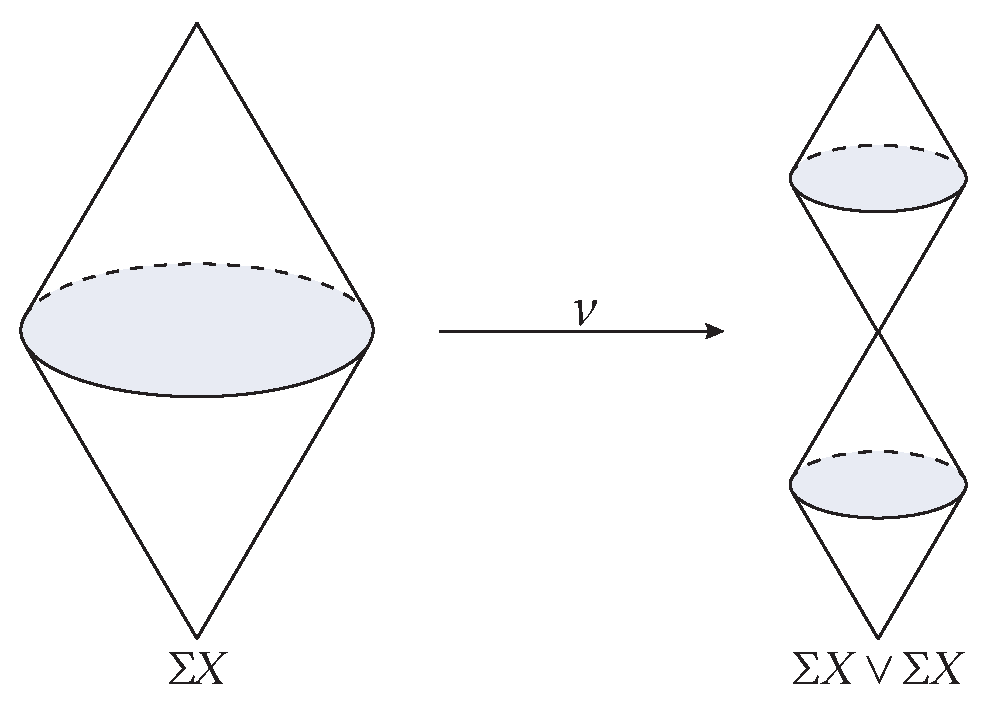
\includegraphics[width=0.45\textwidth]{images/suspoperac.pdf}
\end{figure}

\par
que resulta ser ``co-asociativa'' con ``co-elemento neutro'' y con ``co-elemento inverso'' homotópico:
\begin{prop}
\begin{enumerate}
\item Asociatividad:
\begin{tikzcd}
	\Sigma X \rar{\nu} \dar{\nu} & \Sigma X \vee \Sigma X \dar{1 \vee \nu} \\
	\Sigma X \vee \Sigma X \rar{\nu \vee 1} & \Sigma X \vee \Sigma X \vee \Sigma X
\end{tikzcd}
\item Elemento neutro:
\begin{tikzcd}
	\Sigma X \rar{\nu} \arrow[bend right = 20]{rrr}{1}
 		& \Sigma X \vee \Sigma X \rar{c_{x_0} \vee 1} & \Sigma X \vee \Sigma X \rar{\sigma} & \Sigma X
\end{tikzcd}
\item Elemento inverso:
\begin{tikzcd}
	\Sigma X \rar{\nu} \arrow[bend right = 20]{rrr}{c_{x_0}}
		& \Sigma X \vee \Sigma X \rar{1 \vee \eta} & \Sigma X \vee \Sigma X \rar{\sigma} & \Sigma X
\end{tikzcd}
donde $\eta : \Sigma X \longrightarrow \Sigma X \text{,	} \eta[x,t] = [x, 1-t]$
\end{enumerate}
\end{prop}
Esta co-operación define en $[\Sigma X, Y]$ una operación
\[
\begin{tikzcd}
\Sigma X \rar{\nu} & \Sigma X \vee \Sigma X \rar{f \vee g} & Y \vee Y \rar{\sigma} & Y
\end{tikzcd}
\]
que por la proposición anterior implica:
\begin{teor}
$[\Sigma X, Y]$ es un grupo.
\end{teor}
Y es fácil ver el siguiente resultado.
\begin{teor}
La aplicación $\bar{\varphi} : [\Sigma X, Y] \longrightarrow [X, \Omega Y]$
es un isomorfismo de grupos.
\end{teor}

\subsection{Caso particular grupos de homotopía: $X = S^n$}
Cuando $ X = S^{n-1}$, $\Sigma X \cong S^n$ y al grupo de clases de homotopía punteada
\[ \pi_n(X, x_0) = [S^n, X] \]
se le denomina $n$-ésimo grupo de homotopía de $X$ relativo al punto base $x_0$. \par
La composición es por tanto bastante geométrica:\par \vspace{1em}
\begin{figure}[h]
\centering
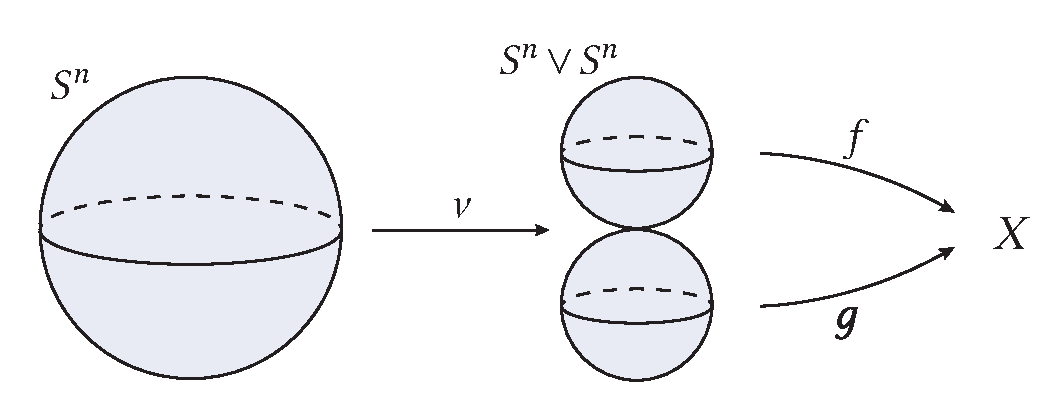
\includegraphics[width=\textwidth]{images/ejgruphomot.pdf}
\end{figure}
\par
Se tiene asímismo, en virtud de todo lo anterior
\begin{teor}
$\pi_n(X) = [S^n, X] = [S^{n-1}, \Omega X] = \pi_{n-1}(\Omega X)$
\end{teor}

\section{CW-complejos}
Es una clase especial de complejos celulares. \par
Sea $X^0$ un espacio topológico discreto: las $0$-celdas. Adjuntamos $I_1$ $1$-celdas a $X^0$ para formar el $1$-esqueleto.
\[ X^1 = X^0 \cup_{\{f_\alpha\}} \left( \dot{\cup} \, e_\alpha^1 \right) \]
Inductivamente, suponemos construido el $(n-1)$-esqueleto $X^{n-1}$ al que adjuntamos una familia de $n$-celdas $\{e_\alpha^n\}_{\alpha \in I_n}$ mediante las correspondientes aplicaciones de adjuncion $f_\alpha : S^{n-1} \longrightarrow X^{n-1}$. \par 
Tenemos entonces dos opciones: el proceso se detiene en un $n$, en cuyo caso la topología ya está definida, o podemos seguir indefinidamente en la sucesion
\[ X^0 \subset X^1 \subset \ldots \subset X^n \subset \ldots \]
y consideramos $ \displaystyle X = \cup_{n \geq 0} X^n $ al que asignamos la topología débil heredada de los esqueletos, esto es $A \subset X$ es abierto si y sólo si $A \cap X^n$ es abierto de $X^n$ para todo $n \geq 0$. \par 
A todo espacio $X$ así construido se le denomina CW-complejo.
\begin{ejems}
\begin{itemize}
\item[(1)] Una superficie orientable compacta $M_g$ de género $g$ ($ g \geq 1$) puede ser construida a partir de un polígono de $4g$ lados identificando los lados de forma que se alternan pares de éstos. Para más claridad, a continuación se presentan algunos casos: \par
\begin{figure}[h]
\centering
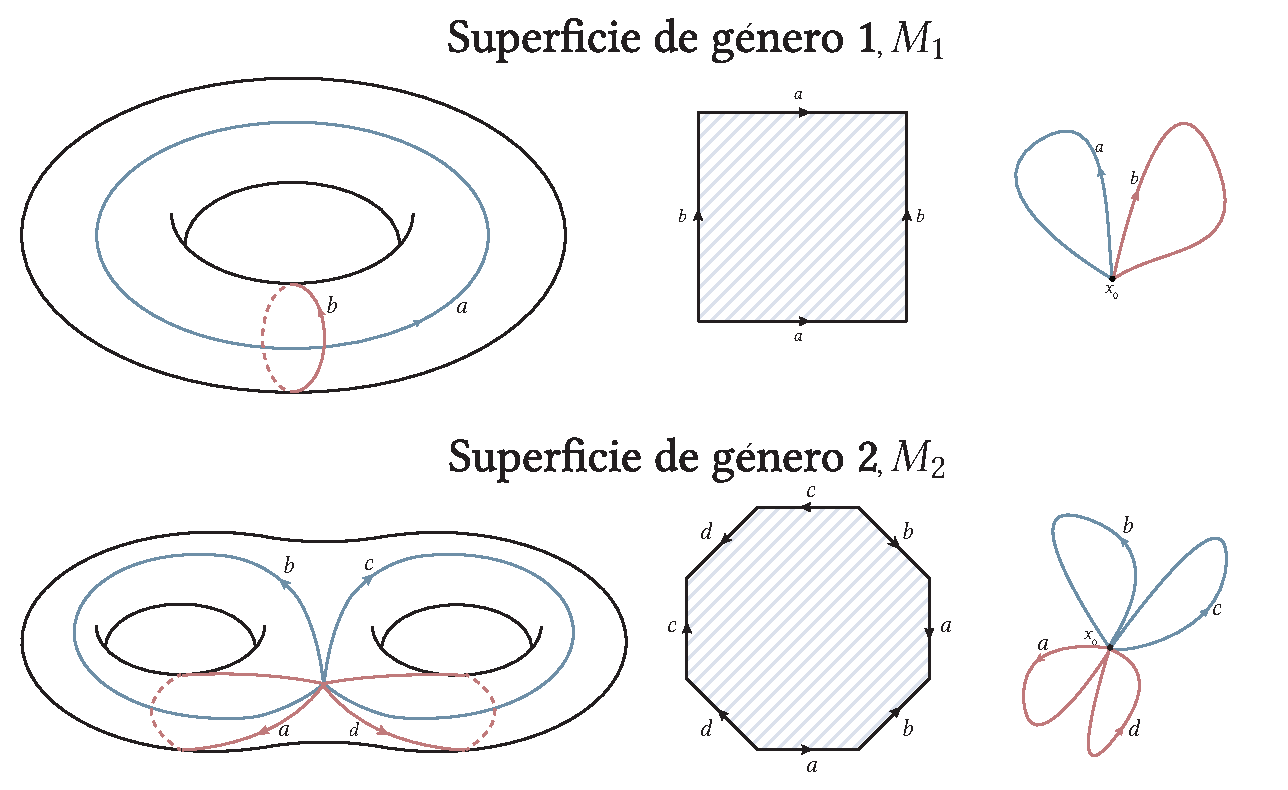
\includegraphics[width=\textwidth]{images/supgeng.pdf}
\end{figure} 
\par 
Con estas identificaciones, los $4g$ lados del polígono se transforman en $2g$ circunferencias unidas por un punto, esto es, adjuntar a $X^0 = \{ \ast \}$ $2g$ $1$-celdas mediante la única posible aplicación de adjunción $S^0 \longrightarrow X^0$. Así pues, $M_g = X^2$ con 
\begin{align*} 
X^0 &= \{ \ast \} \text{,  } X^1 = \bigvee_{2g} S^1 \\
M_g &= X^2 = X^1 \cup_f e^2
\end{align*}

\item $S^n$ tiene estructura de CW-complejo con $1$ $0$-celda y $1$ $n$-celda.
\item El espacio proyectivo real $\mathbb{R}P^n = \faktor{\bb{R}-\{0\}}{\sim}$ donde la relación $\sim$ viene dada por $x \sim y$ si $\exists \lambda \neq 0$ tal que $\lambda x = y$. La aplicación 
\begin{align*}
\bb{R}^{n+1} - \{0\} &\longrightarrow S^n \\
x &\longmapsto \frac{x}{\|x\|}
\end{align*}
induce un homeomorfismo
\[ \bb{R}P^n = \faktor{\bb{R}^{n+1} -\{0\}}{\sim} \stackrel{\cong}{\longrightarrow} \faktor{S^n}{x \sim -x} \]
Por otra parte, la inclusión de un hemisferio $S_+^n \longhookrightarrow S^n$ también induce de forma obvia un homeomorfismo $\faktor{S_+^n}{\sim} \stackrel{\cong}{\longrightarrow} \faktor{S^n}{\sim}$ donde $x \in S^{n-1} \sim \nobreak -x$ \par
\begin{figure}[h]
\centering
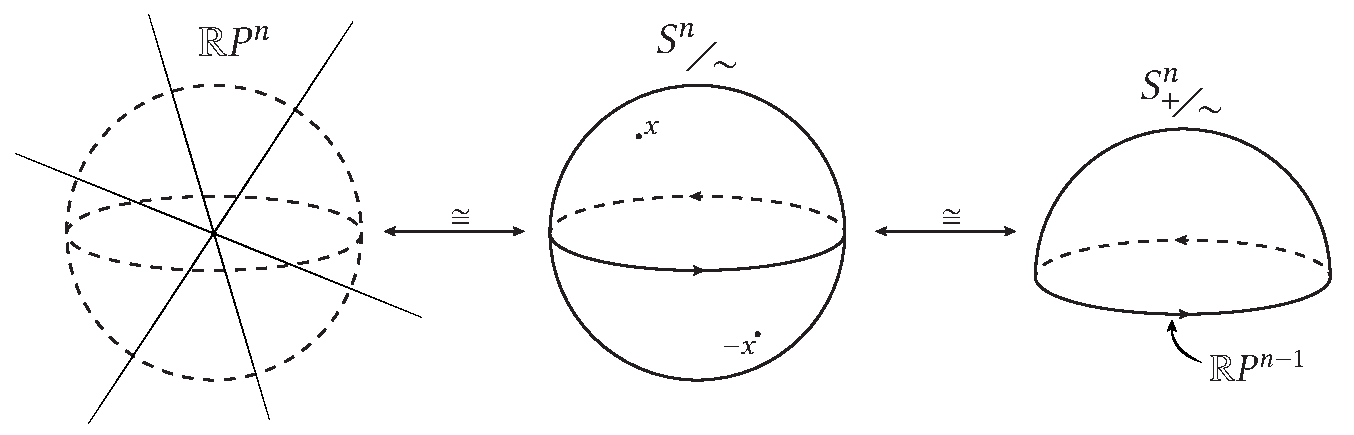
\includegraphics[width=\textwidth]{images/proyecreal.pdf}
\end{figure}
\par 
Así vemos que $\bb{R}P^n = \bb{R}^{n-1} \cup_p e^n$, con $p : S^{n-1} \longrightarrow \bb{R}P^{n-1}$ la proyección. De esta forma $\bb{R}P^n$ admite una estructura con una $i$-celda, $i = 0, 1, \ldots ,n$. \par 
De igual forma $\bb{R}P^\infty = \bigcup_n \bb{R}P^n$ es un CW-complejo con una celda de cada dimensión. $\bb{R}P^\infty$ puede entenderse como las líneas en $\bb{R}^n$ que pasan por el origen.
\end{itemize}
\textbf{Nota:} Si $\varphi : E^n \longhookrightarrow X \dot{\cup} e^n \longrightarrow X \cup_f e^n$ es la aplicación característica de la adjunción de una celda, llamaremos a $\varphi(E^n)$ ``celda'' y a su interior ``celda abierta''. Nótese no obstante que en un CW-complejo una ``$n$-celda abierta'' sólo es abierta en el $n$-esqueleto, pero en general no lo es en el complejo.
\end{ejems}

\subsection{Construcciones básicas con CW-complejos}
\textbf{Subcomplejos}: Dado un CW-complejo X, un subcomplejo $A$ de $X$ es un subespacio de $X$ obtenido adjuntando celdas de la CW-estructura y de forma que $A$ sea también CW-complejo. El $n$-esqueleto de un complejo es un subcomplejo; la semiesfera $S_+^n$ es un subcomplejo de $S^n$... \par 
\textbf{Productos}:  Si X e Y son CW-complejos (localmente finitos), entonces $X \times Y$ hereda una estructura de CW-complejo donde:
\[ (X \times Y)^n = \bigcup_{i+j=n} X^i \times X^j \]
Si $e_i$ (resp. $e_j$) es una $i$-celda de $X$ (resp. $j$-celda de $Y$) con $i+j=n$, con aplicación de adjunción $\varphi_i : S^{i-1} \longrightarrow X^{i-1}$ (resp. $\varphi_j : S^{j-1} \longrightarrow X^{j-1}$), consideramos:
\begin{align*} 
e^{i+j} &= e^i \times e^j \text{ donde } \\
S^{n-1} = S^{i+j-1} &= \partial e^{i+j} = \partial e^i \times e^j \ \cup \ e^i \times \partial e^j \\
&= S^{i-1} \times e^j \ \cup \ e^i \times S^{j-1}
\end{align*}

$\varphi_i$ y $\varphi_j$ definen $\psi : S^{n-1} \longrightarrow (X \times Y)^{n-1}$ dada por 
\[ \psi = \begin{cases}
\varphi_i  \times \phi_j & \text{ en } S^{i-1} \times e^j \\
\phi_i \times \varphi_j & \text{ en } e^i \times S^{j-1}
\end{cases} \]
donde $\phi_i$ y $\phi_j$ son las aplicaciones características. \par 
\textbf{Cocientes}: Si $(X, A)$ es un CW-par ($A$ es un subcomplejo de $X$) el cociente $\faktor{X}{A}$ hereda de forma natural una estructura de CW-complejo. Las celdas de $\faktor{X}{A}$ son las de $X - A$ más una $0$-celda nueva, la imagen de $A$ en $\faktor{X}{A}$. Para cada $n$-celda $e^n$ en $X - A$ con adjunción $\varphi : S^{n-1} \longrightarrow X^{n-1}$ la corespondiente adjunción en $\faktor{X}{A}$ es $S^{n-1} \longrightarrow X^{n-1} \longrightarrow \faktor{X^{n-1}}{A^{n-1}}$. \par
Por ejemplo, si en $S^{n-1}$ tomamos cualquier CW-estructura y construimos $D^n$ adjuntando una $n$-celda a $S^{n-1}$. $\faktor{D^n}{S^{n-1}} = S^n$ con la estructura usual. Otro ejemplo, si en la superficie de género $g$, $M_g$ ``colapsamos'' el $1$-esqueleto $\faktor{M_g}{M_g^1} = S^2$. \par 
Nótese también que $\faktor{X^n}{X^{n-1}} = \bigvee_\alpha S_\alpha^n$ con $\alpha$ variando en el número de $n$-celdas. \par 
\textbf{Wedge y Smash}: Si $\{X_\alpha \}_{\alpha \in I}$ son CW-complejos y $x_0^\alpha \in X_\alpha$  son $0$-celdas, el wedge $\bigvee_{\alpha \in I} X_\alpha$ obtenido al identificar puntos $\{x_0^\alpha \}$ no es más que el cociente $\faktor{\dot{\cup} X_\alpha}{\{x_0^\alpha\}}$ y tiene por lo anterior estructura de CW-complejo. \\
Por otra parte, el smash de $2$ espacios $X$ e $Y$  se define como $X \wedge Y = \faktor{X \times Y}{X \vee Y}$ entendiendo $X \vee Y = X \times \{y_0\} \cup \{x_0\} \times Y$. Si $x_0$ e $y_0$ son $0$-celdas de $X$ e $Y$ respectivamente, entonces $X \times \{y_0\} \cup \{x_0\} \times Y$ es un subcomplejo de $X \times Y$ y podemos tomar el cociente considerando la estructura cociente $X \wedge Y$. \\
Por ejemplo, $S^m \wedge S^n = \faktor{S^m \times S^n}{S^m \vee S^n}$ tiene pues una $0$-celda y una $(n+m)$-celda, por lo cual $S^m \wedge S^n = S^{m+n}$. En particular, $S^1 \wedge S^1 = \faktor{T^2}{S^1 \vee S^1} = S^2$ \nts{Insertar imagen p 33} \par 
\textbf{Espacios de aplicaciones}: SI $X$ es un CW-complejo con finitas celdas e $Y$ tiene un número numerable de ellas, entonces los espacios
$map(X,Y)$, $map_x(X,Y)$, $Y^X$ ó $(Y, y_0)^{(X, x_0)}$ tienen el tipo de homotopía de CW-complejos. En los espacios de aplicaciones tomamos siempre la topología compacto abierta, es decir, la que tiene por subbase a los conjuntos 
\[ \langle K, \theta \rangle = \{f:X \longrightarrow Y : f(K) \subset \theta \} \]
\nts{Añadir nota de p33, demost por Milnor}